\documentclass[11pt,compress,t,notes=noshow, aspectratio=169, xcolor=table]{beamer}

\usepackage{../../style/lmu-lecture}
% Defines macros and environments
 
%\title{iML: Ante-hoc Methods for Neural Networks}
%\subtitle{Motivation}

\title{Interpretable Machine Learning}
\date{}
\begin{document}
%	\maketitle
	\graphicspath{ {./figure/} }

 
\newcommand{\titlefigure}{figure/bild2}
\newcommand{\learninggoals}{
\item Interpretability by sparsity
\item Regularisation for interpretability
\item Sequential feature selection}

\lecturechapter{Ante-hoc Methods for Neural Networks}
\lecture{Interpretable Machine Learning}


\begin{frame}{Motivation}
    \begin{itemize}
        \item Post-hoc methods do not always give you the entire picture
        \item Post-hoc methods are not always accurate
        \begin{itemize}
            \item An explanation that is 10\% inaccurate leads to lack of trust in the ML model
            \item Hard to measure the accuracy of post-hoc methods
        \end{itemize}
        \item Wherever possible use models that are interpretable-by-design
    \end{itemize}
    \begin{figure}
        \centering
        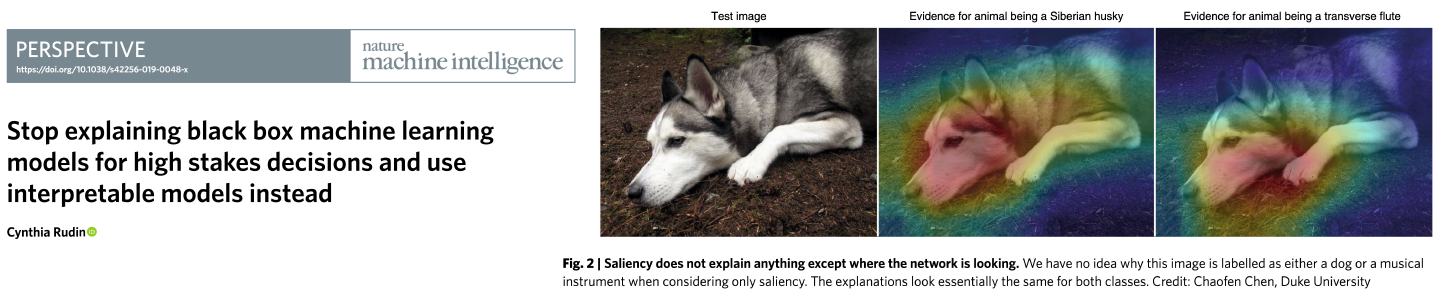
\includegraphics[scale=.4]{bild1}
    \end{figure}
\end{frame}

\begin{frame}{Simpler Models}
    \begin{columns}
    \begin{column}{0.5\textwidth}
    \begin{itemize}
        \item Models that have an understandable decision-making process
        \item Models that have a smaller set of parameters or weights
        \begin{itemize}
            \item Examples: Linear models, GAMs
        \end{itemize}
        \item Models that have human-understandable decision structure
        \begin{itemize}
            \item Examples: decision trees, random forests
        \end{itemize}
        \item Models that have sparsity or only a few set of parameters or features that matter
        \begin{itemize}
            \item Example: 1\% of a large feature space, 1-hot encodings in language tasks
        \end{itemize}
    \end{itemize}
    \end{column}
    \begin{column}{0.5\textwidth}
    \begin{figure}
        \centering
        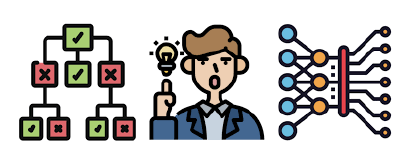
\includegraphics[scale=.7]{bild2}
    \end{figure}
    \end{column}
    \end{columns}
\end{frame}

\begin{frame}[c]{Interpretable by Design Models - Sparse Models}
\begin{itemize}
    \item Models that have explicitly enforce sparsity
    \begin{itemize}
        \item through regularisation
        \item through feature selection
    \end{itemize}
    \bigskip
    \item Sparsity through regularisation
    \begin{itemize}
        \item E.g. L0, L1 regularisation
    \end{itemize}
    \bigskip
    \item Sparsity through feature selection
    \begin{itemize}
        \item select a subset of impacting features for the prediction task
    \end{itemize}
\end{itemize}
    
\end{frame}

\begin{frame}{Regularisation in Neural Networks}
\begin{itemize}
    \item L0 norm is the number of non-zero parameters — setting weights to 0
    \item L1 sparsity — sum of the weights should be small
\end{itemize}

$$
$$
\centerline{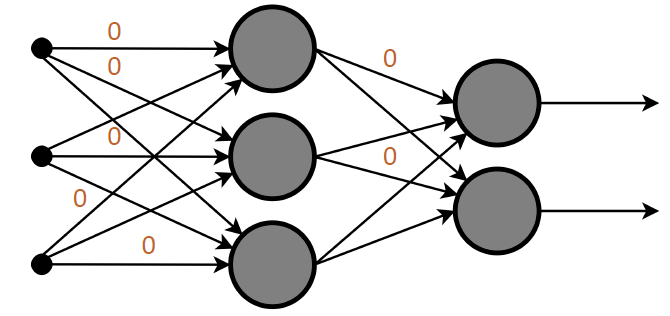
\includegraphics[width=0.5\linewidth]{bild3}}

\end{frame}

\begin{frame}{L1 Regularisation}
    \begin{itemize}
        \item Optimising using L0 regularisation is hard
        \item L1 regularisation in neural networks can be achieved by gradient-based optimisation
        \item Degree of regularisation is a user-controllable parameter
    \end{itemize}
   
   \begin{align*}
       \mathcal{\hat{L}}(W) &= \alpha\|W\|_1 + \mathcal{L}(W)\\
       \nabla_W\mathcal{\hat{L}}(W) &= \alpha sign(W) + \nabla_W\mathcal{L}(W)
   \end{align*}
 
    %\begin{figure}
     %   \centering
      %  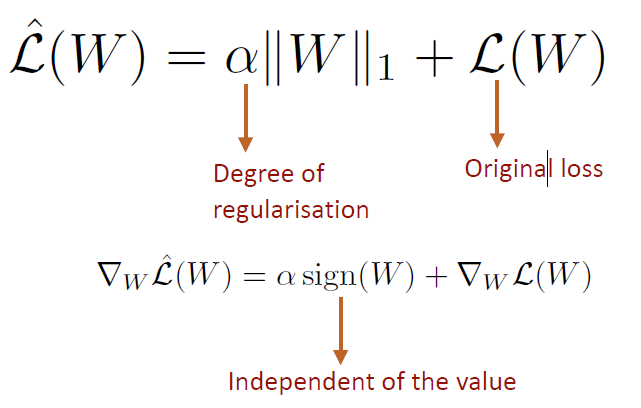
\includegraphics[scale=.4]{bild4}
    %\end{figure}
\end{frame}

\begin{frame}{Feature Selection}
    “Select a smaller features space which can efficiently describe the input data while reducing effects from noise or
irrelevant variables and still provide good prediction results”
\bigskip
    \begin{itemize}
        \item Wrapper methods - Treat the model as a blackbox
        \item Filter methods
        \item Embedded methods
        \item Other methods
        \bigskip
        \item Smaller feature space: subset of features, an embedded hyperspace
    \end{itemize}
\end{frame}

\begin{frame}{Sequential Feature Selection}
\begin{itemize}
    \item Number of feature subsets is $2^N$
    \item How do we reduce the computational complexity of checking each subset ?
    \begin{itemize}
        \item Sequentially choose the most promising feature at each iteration
    \end{itemize}
    \bigskip
    \item Selection Set S= \{\}, All features N= $\{f_1,f_2, \dots , F_n\}$
    \item In each iteration
    \begin{itemize}
        \item compute utility of f- train a model with S $\cup\{f\}$ and measure validation perf.
        \item terminate loop if no improvement of utility and return S
        \item choose f in N/S that has max utility and add f to S
    \end{itemize}
\end{itemize}
    
\end{frame}
\begin{frame}{Feature Selection}
\begin{itemize}
    \item What are the short comings of sequential feature selection ?
    \begin{itemize}
        \item Greedy might not be optimal
        \item Global feature selection method
    \end{itemize}
    \bigskip
    \item How do we improve the greedy solution ?
     \begin{itemize}
        \item Allow for backtracking, branch-and-bound
        \item Use genetic algorithms GA, swarm optimisation
    \end{itemize}
    \bigskip
    \item How do we choose a local feature selection method ?
    \begin{itemize}
        \item instance-wise feature selection methods
    \end{itemize}
\end{itemize}
    
\end{frame}

\endlecture
\end{document}